% Rendered automatically from content.tex.in + data/canonical_results.json
% DO NOT EDIT NUMBERS BY HAND -- edit templates or code and re-run render_manuscript.py.

\section{Introduction}

Multiplex polymerase chain reaction (multiplex PCR) simultaneously amplifies dozens to hundreds of genomic loci in a single reaction volume for targeted next-generation sequencing (NGS), clinical oncology panels, and pathogen surveillance\supercite{untergasser2012primer3}. Scaling to high plexities is constrained by pairwise primer--primer cross-hybridization: pooling $2N$ primers for $N$ targets creates $\binom{2N+1}{2} = N(2N+1)$ unordered candidate interactions (including homodimers). Extensible $3'$-terminal complementarity produces short artifactual primer-dimers that amplify faster than genomic targets and deplete on-target sequencing depth\supercite{xie2022designing}.

To mitigate this interaction burden, \citet{xie2022designing} introduced SADDLE (\emph{Simulated Annealing Design using Dimer Likelihood Estimation}), combining an empirical biophysical \emph{Badness} heuristic with simulated annealing optimization. In their empirical NGS validation on an Illumina MiSeq (MiSeq Reagent Kit v2), primer-dimer reads in a 96-plex cancer-exon panel dropped from 90.7\% in an unoptimized pool (PS1) to 39.6\% at an intermediate generation (PS2) and 4.9\% in the optimized pool (PS3; Figure~3a). Scaling to a 384-plex human SNP panel (768 primers; Sample~E19; Figure~3f), the authors reported approximately 43\% on-target amplicons, roughly 56\% nonspecific amplicons, and about 1\% primer-dimers.

Reproducing these empirical NGS analyses from the primary sequencing data presents two practical barriers:
\begin{enumerate}
  \item \textbf{Commercial software and panel-size hardcoding:} Under \emph{Code availability}, \citet{xie2022designing} state verbatim: \emph{``The MATLAB code used for multiplex PCR primer algorithm is available upon request under NDA for academic lab. The MATLAB code and Python code for NGS data processing are available at \url{https://github.com/NinaGXie/SADDLE}.''} Under \emph{Competing interests}, a patent on the primer design algorithm was reported as pending in \citet{xie2022designing} (exclusively licensed to NuProbe Global; post-2022 legal status was not independently audited). While the NGS scripts (\texttt{Data\_process.m}, \texttt{Dimer\_Identify.m}, \texttt{analysis\_code.ipynb}) and 96-plex Bowtie2 references (\texttt{Ref\_1.fasta}--\texttt{Ref\_3.fasta}) are public, executing them requires commercial MATLAB (with Bioinformatics Toolbox \texttt{swalign}), \texttt{Dimer\_Identify.m} is hardcoded to 192 primers (96-plex), and no 384-plex reference FASTA is provided.
  \item \textbf{Unreported denominators and provenance ambiguities:} Figures~3a and~3f report percentage summaries without integer read denominators or exclusion counts, and the Figshare archive (\doi{10.6084/m9.figshare.16944154.v3})\supercite{xie2021figshare} does not specify whether the E14 PS1--PS3 FASTQ files correspond to the concentration-optimized or non-optimized libraries in Supplementary Data~3 (\texttt{MOESM7}).
\end{enumerate}

Following ReScience~C guidelines\supercite{rougier2017sustainable}, we present an independent open-source reimplementation of selected primary empirical NGS validation analyses from \citet{xie2022designing} across four panels (PS1, PS2, PS3, and E19; 9,456,130 raw paired-end reads). Because SADDLE's simulated annealing primer-design algorithm is not publicly released, primer-pool optimization is outside our scope; this work is therefore a \textbf{partial computational replication} focused on Figures~3a and~3f and Supplementary Data~3. Specifically, we:
\begin{itemize}
  \item Reimplement the reported NGS workflow (\texttt{Data\_process.m} $\rightarrow$ Bowtie2 $\rightarrow$ \path{analysis_code.ipynb} $\rightarrow$ \texttt{Dimer\_Identify.m}) in open-source Python and Bowtie2\supercite{langmead2012fast} (\textbf{Pipeline~A}), eliminating commercial MATLAB dependencies and scaling to both 96-plex and 384-plex.
  \item Benchmark a standalone Python/\texttt{edlib}\supercite{sosic2017edlib} pipeline requiring no external command-line aligner (\textbf{Pipeline~B}) across 75\%/80\%/85\% similarity thresholds alongside Pipeline~A.
  \item Archive all six reconstructed 96-plex directional and unordered pair tables and validate them cell-by-cell against Supplementary Data~3 (\texttt{MOESM7}) using correlation, active-pair exact agreement, Jaccard, count-stratified disagreement, and normalized L1 error metrics, while characterizing heavy-tailed dimer concentration in E19.
  \item Perform a matched-pair alignment audit on a seeded uniform random sample ($N = 5,000$) comparing Bowtie2, cognate-anchored \texttt{edlib}, and all-target \texttt{edlib} on identical read pairs with full per-read audit tables and Wilson 95\% confidence intervals, plus a seeded indel recovery audit ($N = 20,000$).
\end{itemize}

\section{Original Artifacts and Replication Methodology}

\subsection{Primary Data, Input Integrity, and Reference Construction}

All raw sequencing files were retrieved from Figshare (\doi{10.6084/m9.figshare.16944154.v3}, CC~BY~4.0; author: Nina Xie; live API metadata snapshot in \path{data/figshare_v3_metadata_snapshot.json})\supercite{xie2021figshare} and verified programmatically against pinned URLs, byte sizes, and SHA-256 checksums (\path{data/expected_raw_sha256.json}, automated via \path{code/download_raw_data.py}) before processing:
\begin{itemize}
  \item PS1 (96-plex, Figure~3a): \path{SADDLE_PS1_E14_Raw_R1/R2.fastq.gz} (1,823,058 pairs);
  \item PS2 (96-plex, Figure~3a): \path{SADDLE_PS2_E14_Raw_R1/R2.fastq.gz} (1,952,269 pairs);
  \item PS3 (96-plex, Figure~3a): \path{SADDLE_PS3_E14_Raw_R1/R2.fastq.gz} (1,738,418 pairs);
  \item E19 (384-plex, Figure~3f): \path{E19_384plex_NGS_R1/R2_fastq.gz} (3,942,385 pairs).
\end{itemize}
Paired FASTQ streaming enforces mate-ID synchronization, equal sequence and quality lengths, valid record headers, and EOF parity. Primer sequences and 384-plex genomic contexts were read from Supplementary Data~1 (\path{41467_2022_29500_MOESM5_ESM.xlsx}), and published 96-plex dimer matrices from Supplementary Data~3 (\path{41467_2022_29500_MOESM7_ESM.xlsx}). Licensing and third-party provenance for all components are documented separately in \path{DATA_AND_LICENSES.md}.

For PS1--PS3, because the upstream repository lacks an explicit license header, \path{Ref_1.fasta}--\path{Ref_3.fasta} are not redistributed in this archive; instead, \path{code/download_raw_data.py} retrieves them programmatically from pinned commit \texttt{1e474abf88f0} of \texttt{NinaGXie/SADDLE} and verifies their exact SHA-256 digests and 96/96 exact $5'$ forward and $3'$ reverse-complement primer boundaries against \texttt{MOESM5}. For E19, all 384 amplicons were strictly extracted from the 1,001-bp contexts in \texttt{MOESM5} (\texttt{384 Plex Info}), raising an error if any primer boundary is absent (384/384 exact extractions). We note a minor typographical discrepancy in \citet{xie2022designing}: the Introduction once states ``784 primers (384-plex),'' whereas the Abstract, Figure~3f, and \texttt{MOESM5} confirm 384 forward + 384 reverse = 768 primers.

\subsection{Pipeline A (Python + Bowtie2) and Pipeline B (Standalone Python/\texttt{edlib})}

Table~\ref{tab:mapping} maps the original scripts to our two open-source pipelines (tested on Python 3.12.4, bowtie2 2.5.5, and \texttt{edlib} 1.3.9.post1; locked dependencies are provided in \path{environment.yml} and \texttt{requirements-\allowbreak lock-\allowbreak py312.txt}, with cross-version bounds in \path{requirements.txt}). Note that \texttt{edlib} is a C/C++ library accessed via Python bindings\supercite{sosic2017edlib}; Pipeline~B is therefore a standalone Python/\texttt{edlib} workflow without an external command-line aligner.

\begin{table}[!htbp]
\centering
\caption{Structural mapping between the original SADDLE NGS scripts and our two open-source reimplementations.}
\label{tab:mapping}
\scriptsize
\setlength{\tabcolsep}{3.5pt}
\begin{tabular}{@{}p{1.8cm}p{3.6cm}p{3.7cm}p{3.4cm}@{}}
\hline
\textbf{Stage} & \textbf{Original SADDLE} & \textbf{Pipeline A (Python + Bowtie2)} & \textbf{Pipeline B (Python/\texttt{edlib})} \\
\hline
Adapter trim & \texttt{Data\_process.m}: 28-bp R1/R2 adapters; require both mates. & Same 28-bp R1/R2 adapters; require both mates. & Core 17-bp TruSeq R1/R2 prefixes; require both mates. \\
Quality filter & \texttt{Data\_process.m}: len $>10$~bp, no \texttt{N}, $>70\%$ Phred $>30$. & Reimplementation ($>10$~bp, no \texttt{N}, $>70\%$ Q30). & Reimplementation ($>10$~bp, no \texttt{N}, $>70\%$ Q30). \\
Length split & Both $\ge 60$~bp $\rightarrow$ Bowtie2; both $<60$~bp $\rightarrow$ \texttt{DimerCand}. & Same 60-bp split; logs mixed-length drops explicitly. & Single-stream; no 60-bp length split. \\
On-target call & \texttt{bowtie2} paired-end + \texttt{analysis\_code.ipynb} (\texttt{mapped//2}). & Open-source \texttt{bowtie2} (bowtie2 2.5.5) + SAM parser tracking \texttt{mapped//2} and both-mapped pairs. & M1: cognate primers ($P_2{=}P_1{+}N$). M2: \texttt{edlib} SHW ($\ge 75\%, 80\%, 85\%$). \\
Primer match \& dimers & \texttt{Dimer\_Identify.m}: len$>15$, len$(p)\le$len$(r)$, 8-bp hash, MATLAB \texttt{swalign} $>0.6$, insert $<L_1{+}L_2{-}2$; hardcoded 96-plex. & len$>15$, len$(p)\le$len$(r)$, 8-bp hash, Smith--Waterman NUC44 ($+5/{-}4/{-}8$) ratio $>0.6$, insert $<L_1{+}L_2{-}2$; scaled to $2N{\times}2N$. & 8-bp hash; positional identity $>0.6$ over $\min(|p|,|r|)$; insert $<L_1{+}L_2{-}2$. \\
\hline
\end{tabular}
\end{table}

Auditing the original scripts revealed two edge cases logged explicitly by Pipeline~A: (i) \texttt{Data\_process.m} (lines~118--128) silently drops mixed-length pairs where one mate is $\ge 60$~bp and the other $< 60$~bp; and (ii) \texttt{analysis\_code.ipynb} (line~16) estimates mapped pairs via integer floor division (\texttt{OnTar = df.mapped // 2}), i.e., $N_{\mathrm{on}} = \lfloor(2B + H)/2\rfloor = B + \lfloor H/2\rfloor$, where $B$ is pairs with both mates mapped and $H$ is singly mapped pairs, thereby adding $\lfloor H/2\rfloor$ pairs to the aggregate on-target count while routing only both-unmapped pairs to \texttt{Dimer\_Identify.m}. Because we did not execute commercial MATLAB side-by-side, Pipeline~A's Smith--Waterman routine is described strictly as an open-source reimplementation using the documented NUC44 ($+5/-4/-8$) scoring scheme rather than a proven line-for-line MATLAB identity.

\section{Replication Results}

\subsection{Multi-Panel Read Partitions Across PS1--PS3 (Figure 3a) and E19 (Figure 3f)}

Table~\ref{tab:multipanel} and Figure~\ref{fig:multipanel} compare our replicated read partitions against the published figures of \citet{xie2022designing}:
\begin{itemize}
  \item \textbf{96-Plex Optimization Trajectory (Figure~3a):} Under Pipeline~A, primer-dimer fractions drop from \textbf{90.66\%} in PS1 (published: 90.7\%, $\Delta = -0.04$~pp) to \textbf{39.62\%} in PS2 (published: 39.6\%, $\Delta = +0.02$~pp) and \textbf{4.97\%} in PS3 (published: 4.9\%, $\Delta = +0.07$~pp), while on-target rates rise from 2.65\% to 32.78\% and 66.16\%. Our PS1 on-target pair count (36,243) closely matches the saved cell output (\texttt{36203}) in the authors' \texttt{analysis\_code.ipynb} for \texttt{E14\_Lib1} (0.11\% difference).
  \item \textbf{384-Plex Validation Panel (Sample~E19, Figure~3f):} Pipeline~A yields \textbf{42.76\%} on-target (1,190,632 pairs), \textbf{56.39\%} nonspecific (1,570,289 pairs), and \textbf{0.85\%} primer-dimers (23,534 pairs) over 2,784,455 classified pairs. Rounded to integers, these equal \textbf{43\% / 56\% / 1\%}, agreeing with Figure~3f.
  \item \textbf{Edge-case and raw-denominator accounting:} Mixed-length 60-bp drops affect only 117 (PS1), 25 (PS2), 5 (PS3), and 1 (E19) pairs; integer floor division of singly mapped pairs ($H = 2, 19, 46, 238$) adds $\lfloor H/2\rfloor = 1, 9, 23, 119$ pairs ($<0.003$~pp impact; strict both-mapped E19 on-target = 42.76\%). Over \emph{total raw sequencer output}, Pipeline~A excludes 25.02\% (PS1), 24.71\% (PS2), 29.14\% (PS3), and 29.37\% (E19) of raw pairs; on-target raw shares are 1.99\%, 24.68\%, 46.88\%, and 30.20\% (E19 dimers: 0.60\% of raw reads).
\end{itemize}

\begin{table}[!htbp]
\centering
\caption{Multi-panel replication of SADDLE empirical NGS read partitions across PS1--PS3 (Figure~3a) and E19 (Figure~3f). Analysis denominator is classified read pairs, except for the E19 Raw Basis row, which uses total raw read pairs.}
\label{tab:multipanel}
\scriptsize
\setlength{\tabcolsep}{2.8pt}
\begin{tabular}{@{}llrrrrrr@{}}
\hline
\textbf{Panel} & \textbf{Pipeline / Criterion} & \textbf{Raw Pairs} & \textbf{Analysis Denom.} & \textbf{On-Target} & \textbf{Nonspec.} & \textbf{Dimers} & \textbf{Published} \\
\hline
PS1 (96) & Pipeline A (Bowtie2) & 1,823,058 & 1,366,868 & 2.65\% & 6.68\% & \textbf{90.66\%} & 90.7\% dim. \\
PS1 (96) & Pipeline B (\texttt{edlib} $\ge 75\%$) & 1,823,058 & 1,438,981 & 2.32\% & 6.82\% & 90.87\% & 90.7\% dim. \\
\hline
PS2 (96) & Pipeline A (Bowtie2) & 1,952,269 & 1,469,910 & 32.78\% & 27.60\% & \textbf{39.62\%} & 39.6\% dim. \\
PS2 (96) & Pipeline B (\texttt{edlib} $\ge 75\%$) & 1,952,269 & 1,490,033 & 29.59\% & 29.07\% & 41.34\% & 39.6\% dim. \\
\hline
PS3 (96) & Pipeline A (Bowtie2) & 1,738,418 & 1,231,925 & 66.16\% & 28.87\% & \textbf{4.97\%} & 4.9\% dim. \\
PS3 (96) & Pipeline B (\texttt{edlib} $\ge 75\%$) & 1,738,418 & 1,218,237 & 61.71\% & 32.95\% & 5.34\% & 4.9\% dim. \\
\hline
E19 (384) & Pipeline A (Bowtie2) & 3,942,385 & 2,784,455 & \textbf{42.76\%} & \textbf{56.39\%} & \textbf{0.85\%} & $\sim$43/56/1\% \\
E19 (384) & Pipeline B, M1 (Primer) & 3,942,385 & 2,860,664 & 43.86\% & 55.27\% & 0.87\% & $\sim$43/56/1\% \\
E19 (384) & Pipeline B, \texttt{edlib} $\ge 75\%$ & 3,942,385 & 2,860,664 & 43.59\% & 55.54\% & 0.87\% & $\sim$43/56/1\% \\
E19 (384) & Pipeline B, \texttt{edlib} $\ge 80\%$ & 3,942,385 & 2,860,664 & \textbf{42.75\%} & \textbf{56.38\%} & 0.87\% & $\sim$43/56/1\% \\
E19 (384) & Pipeline B, \texttt{edlib} $\ge 85\%$ & 3,942,385 & 2,860,664 & 39.87\% & 59.26\% & 0.87\% & $\sim$43/56/1\% \\
E19 (384) & Pipeline B, Ungap. $\ge 75\%$ & 3,942,385 & 2,860,664 & 39.35\% & 59.78\% & 0.87\% & Ref. \\
E19 (384) & Pipeline A (Raw Basis) & 3,942,385 & 3,942,385 & 30.20\% & 39.83\% & 0.60\% & --- \\
\hline
\end{tabular}
\end{table}

\begin{figure}[!htbp]
\centering
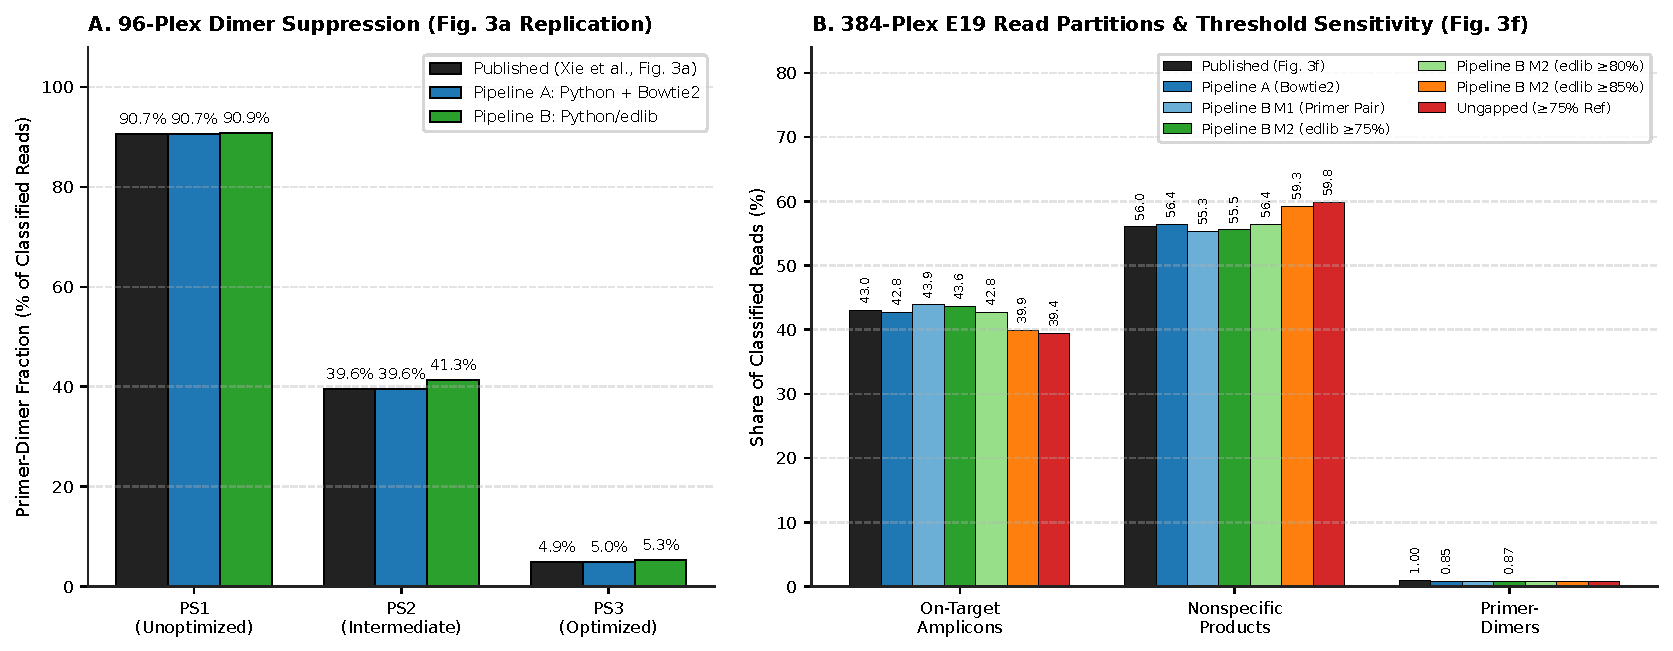
\includegraphics[width=\textwidth]{figures/fig1_multipanel_replication.pdf}
\caption{Multi-panel replication of SADDLE empirical NGS read partitions. \textbf{(A)} 96-plex primer-dimer suppression from PS1 to PS3 (Figure~3a): Pipeline~A (Python + Bowtie2) reproduces 90.7\% $\rightarrow$ 39.6\% $\rightarrow$ 4.9\% within 0.08~pp; Pipeline~B (standalone Python/\texttt{edlib}) captures the same trend with slightly higher dimer fractions due to differing retained read subsets. \textbf{(B)} 384-plex E19 partitions (Figure~3f) across Pipeline~A, Pipeline~B (M1, \texttt{edlib} $\ge 75\%$, $\ge 80\%$, $\ge 85\%$), and ungapped comparison ($\ge 75\%$).}
\label{fig:multipanel}
\end{figure}

\subsection{Comparison of Pipeline A (Bowtie2) and Pipeline B (Standalone Python/\texttt{edlib})}

Two methodological patterns emerge when comparing Pipeline~A and Pipeline~B:
\begin{enumerate}
  \item \textbf{Threshold sensitivity on E19:} Under Pipeline~B, E19 on-target classification decreases monotonically with stringency: 43.86\% (M1) $\rightarrow$ 43.59\% (\texttt{edlib} $\ge 75\%$) $\rightarrow$ 42.75\% (\texttt{edlib} $\ge 80\%$) $\rightarrow$ 39.87\% (\texttt{edlib} $\ge 85\%$), while ungapped matching yields 39.35\%. At $\ge 80\%$, Pipeline~B agrees with Pipeline~A (42.76\%) within 0.01~pp at the aggregate level, though their retained read populations differ (2,860,664 vs. 2,784,455 classified pairs).
  \item \textbf{Divergence on PS2 and PS3:} On PS2 and PS3, Pipeline~B assigns 3.2--4.4~pp fewer on-target reads than Pipeline~A (PS2: 29.59\% vs. 32.78\%; PS3: 61.71\% vs. 66.16\%) and slightly higher dimer fractions (41.34\% vs. 39.62\%; 5.34\% vs. 4.97\%). Pipeline~A aligns long reads with Bowtie2 \emph{before} applying the 8-bp $5'$ primer prefix hash, retaining amplicon reads with minor $5'$ errors, whereas Pipeline~B filters 12.08\% and 12.98\% of raw reads as primer-unmatched. Retaining open-source Bowtie2 therefore tracks the original procedure more closely.
\end{enumerate}

\subsection{Cell-by-Cell Matrix Validation (PS1--PS3) and Heavy-Tailed Concentration (E19)}

To move beyond aggregate percentages, we compared all six reconstructed 96-plex dimer pair tables (archived under \path{data/matrices/} with directional columns \texttt{reads\_p1\_p2} and \texttt{reads\_p2\_p1} alongside unordered totals \texttt{dimer\_reads}, preserving the full ordered $192 \times 192$ matrix and 18,528 unordered pairs) cell-by-cell against both conditions in Supplementary Data~3 (\texttt{MOESM7}; Table~\ref{tab:matrix}, Figure~\ref{fig:dimer}B). Because Pearson correlation can be dominated by high-count pairs and all-cell exact agreement is inflated by structural zeros, Table~\ref{tab:matrix} reports Spearman $\rho$, exact agreement restricted to the active-pair union (\textbf{Act.\ Exact}), active-pair Jaccard overlap, MAE, and normalized L1 total absolute error ($\sum |r_i - p_i| / \sum p_i$).

\begin{table}[!htbp]
\centering
\caption{Cell-by-cell validation of Pipeline~A reconstructed 96-plex dimer matrices (18,528 unordered pairs) against published Supplementary Data~3 (\texttt{MOESM7}). \textbf{Act.\ Exact}: exact integer agreement restricted to the union of active pairs (excluding shared zeros).}
\label{tab:matrix}
\scriptsize
\setlength{\tabcolsep}{2.3pt}
\begin{tabular}{@{}llrrrrrrrr@{}}
\hline
\textbf{Panel} & \textbf{MOESM7 Sheet} & \textbf{Ratio} & \textbf{Pearson $r$} & \textbf{Spearman $\rho$} & \textbf{Act.\ Exact} & \textbf{Jaccard} & \textbf{MAE} & \textbf{Norm.\ L1} & \textbf{Top-10} \\
\hline
PS1 & \texttt{conc opt.} & 0.9972 & \textbf{0.99999} & 0.9361 & 65.6\% & 0.8765 & 0.34 & 0.51\% & 10/10 \\
PS1 & \texttt{not opt.} & 1.4388 & 0.3219 & 0.5458 & 3.0\% & 0.3752 & 76.14 & 163.79\% & 6/10 \\
\hline
PS2 & \texttt{conc opt.} & 0.9986 & \textbf{0.99999} & 0.9048 & 56.7\% & 0.8196 & 0.22 & 0.69\% & 10/10 \\
PS2 & \texttt{not opt.} & 1.3934 & 0.7251 & 0.5852 & 3.3\% & 0.4082 & 26.67 & 118.23\% & 5/10 \\
\hline
PS3 & \texttt{conc opt.} & 1.0067 & \textbf{0.99999} & 0.8722 & 61.9\% & 0.7614 & 0.03 & 1.02\% & 10/10 \\
PS3 & \texttt{not opt.} & 0.3793 & 0.1143 & 0.4898 & 1.2\% & 0.3258 & 10.41 & 119.40\% & 3/10 \\
\hline
\end{tabular}
\end{table}

Against the \texttt{conc optimized} matrices, Pipeline~A achieves Pearson $r = 0.999988$--$0.999992$, normalized L1 error of 0.51--1.02\%, active-pair Jaccard overlap of 0.7614--0.8765, exact integer agreement on 56.7--65.6\% of active-union cells (98.47--99.37\% across all 18,528 cells including shared zeros), total count ratios of 0.9972--1.0067, and 10/10 overlap among the top-10 pairs (Pipeline~B achieves Pearson $r = 0.99998$, $0.99926$, and $0.99978$). Direct count stratification against \texttt{MOESM7} shows that 30.8--50.0\% of disagreeing cells have $\max(\text{rec},\text{pub}) \le 2$ reads (contributing 0.7--12.4\% of total L1 reads), whereas high-count cells ($\ge 10$ reads) contribute 98.6\% (PS1), 94.3\% (PS2), and 76.6\% (PS3) of total L1 count differences despite small fractional offsets. By contrast, correlations with the \texttt{not optimized} matrices are far lower ($r = 0.1143$--$0.7251$ across PS1--PS3), resolving an undocumented provenance detail: the Figshare \texttt{E14} FASTQs correspond to the concentration-optimized PS1--PS3 libraries.

In the 384-plex E19 library, dimer formation across the 295,296 candidate unordered pairs is highly sparse and heavy-tailed (Figure~\ref{fig:dimer}A; no formal power-law fit is claimed). Under Pipeline~B, 294,122 pairs (99.60\%) yield zero dimer reads, 1,174 pairs (0.398\%) exhibit $\ge 1$ read, and 98 pairs (0.0332\%) exhibit $\ge 10$ reads. A single reverse--reverse pair (\texttt{rp213} $\times$ \texttt{rp371}) accounts for 16,805 of 24,878 dimer reads (\textbf{67.55\%}; top-10 pairs: 81.41\%). Under Pipeline~A, the same dominant pair accounts for 16,365 of 23,534 dimer reads (\textbf{69.54\%}) across 1,022 active pairs. Although low-count active pair totals differ between pipelines (1,022 vs. 1,174), the dominant interaction and strong concentration of dimer reads are robust across both pipelines.

\begin{figure}[!htbp]
\centering
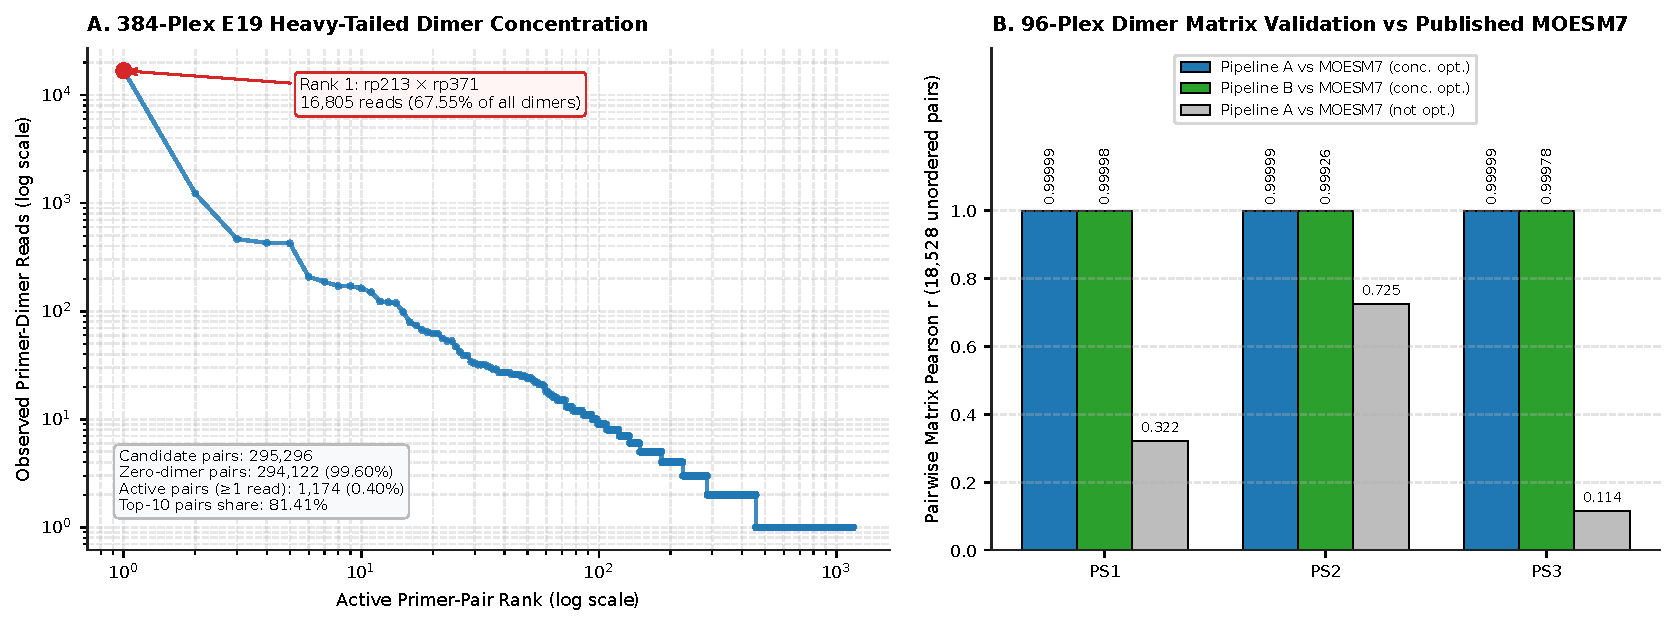
\includegraphics[width=\textwidth]{figures/fig2_dimer_concentration_and_matrix.pdf}
\caption{Pair-level primer-dimer structure and matrix validation. \textbf{(A)} Log-log rank-abundance curve of the 1,174 active dimer pairs in E19 (generated from archived \texttt{data/saddle\_384\_dimer\_pairs.tsv}), showing heavy-tailed concentration in rank-1 pair \texttt{rp213} $\times$ \texttt{rp371} (67.55\%). \textbf{(B)} Cell-by-cell Pearson correlation across all 18,528 unordered 96-plex pairs against published \texttt{MOESM7} sheets, verifying strong matrix agreement ($r \ge 0.999988$ for Pipeline~A) and identifying the Figshare E14 files as the concentration-optimized libraries.}
\label{fig:dimer}
\end{figure}

\subsection{Matched-Pair Uniform Random Audits of Alignment Scope and Indel Recovery}

To avoid tile-order bias and cross-denominator comparisons, we drew a seeded uniform reservoir sample across all 2,835,786 qualifying Pipeline~B non-dimer read pairs in E19 (\texttt{seed=20261124}), evaluated \emph{all three alignment methods on the exact same $N = 5,000$ read pairs}, and archived complete per-read classifications in \path{data/matched_pair_audit_5000.tsv.gz}:
\begin{enumerate}
  \item \textbf{Matched-pair alignment comparison ($N = 5,000$ identical non-dimer pairs):}
  \begin{itemize}
    \item \emph{Paired-end Bowtie2 (on the exact same 5,000 pairs):} Both mates map to the 384-amplicon reference for \textbf{41.26\%} of pairs (2,063/5,000; 95\% Wilson CI: 39.90--42.63\%), identical to the proper-pair concordant set (2,063/5,000, 41.26\%). Exactly 4,684 pairs meet the $\ge 60$~bp length criterion on both mates (41.22\% mapped under $\ge 60$~bp; 316 pairs have at least one mate $<60$~bp).
    \item \emph{Cognate-anchored vs. all-384-target \texttt{edlib} ($\ge 75\%$):} Cognate-anchored = \textbf{44.88\%} (95\% CI: 43.51--46.26\%) vs. dual-strand all-target = \textbf{47.50\%} (95\% CI: 46.12--48.89\%); concordance = 97.38\% (96.90--97.79\%), with 131 non-cognate reads matching a target (all individually auditable in \path{data/matched_pair_audit_5000.tsv.gz}). Among cognate-labelled reads, 0/2,256 strictly better and 0/2,256 tied non-cognate best matches passed the 75\% threshold; across all similarity levels, 2 cognate-labelled reads exhibited slightly higher non-cognate alignments below both acceptance thresholds (59.74--60.26\% vs. 58.44--58.97\%). Against matched paired-end Bowtie2, cognate \texttt{edlib} $\ge 75\%$ achieves 94.54\% concordance (93.88--95.14\%, $\Delta = +3.62$~pp) and all-target \texttt{edlib} $\ge 75\%$ achieves 93.76\% (93.06--94.40\%, $\Delta = +6.24$~pp).
    \item \emph{Cognate-anchored vs. all-384-target \texttt{edlib} ($\ge 80\%$):} Cognate-anchored = \textbf{44.08\%} (95\% CI: 42.71--45.46\%) vs. all-target = \textbf{45.44\%} (95\% CI: 44.06--46.82\%); concordance = 98.64\% (98.28--98.93\%; 0 strictly better and 0 tied non-cognate best matches passing 80\%). Against matched Bowtie2, cognate \texttt{edlib} $\ge 80\%$ achieves 95.34\% concordance (94.72--95.89\%, $\Delta = +2.82$~pp) and all-target \texttt{edlib} $\ge 80\%$ achieves 95.82\% (95.23--96.34\%, $\Delta = +4.18$~pp).
  \end{itemize}
  Single-end \texttt{edlib} classified a larger fraction of the matched read pairs as on-target than paired-end Bowtie2. These differences may reflect differences in mate requirements, alignment scoring, target search, and acceptance thresholds.
  \item \textbf{Gapped vs. ungapped indel recovery ($N = 20,000$ random cognate reads from 1,254,647):} Exactly 1,856 reads (9.28\%, 95\% CI: 8.89--9.69\%) passed gapped \texttt{edlib} ($\ge 75\%$) after failing ungapped positional matching ($\ge 75\%$). Full CIGAR parsing showed that \textbf{100.0\%} (1,856/1,856) contained alignment gaps (0 substitution-only), with 204 (10.99\%) having $\le 2$~bp indels and 1,652 (89.01\%) having $>2$~bp or multi-gap events (median 8.0~bp, IQR 4.0--9.0~bp). This documents alignment gaps under our computational procedure without attributing them to biological insertions or deletions.
\end{enumerate}

\section{Limitations, Verification, and Availability}

Four scope limitations apply. First, 21--30\% of raw sequencing pairs are excluded during adapter trimming, quality filtering, and primer matching, and Pipelines~A and~B retain slightly different read populations (28-bp vs. 17-bp adapter rules and Bowtie2-first vs. primer-first routing); aggregate differences between the two pipelines therefore reflect both alignment logic and retained-read differences. Second, SADDLE's simulated annealing primer-design algorithm is not publicly released and is not replicated here. Third, we did not execute the original scripts inside commercial MATLAB, so minor boundary differences against MATLAB \texttt{swalign} cannot be excluded. Fourth, software engineering and draft manuscript preparation used AI coding assistance, with all quantitative results derived programmatically from \path{data/canonical_results.json} and flagged for independent human verification in \path{data/evidence_claim_ledger_draft.json}.

To verify end-to-end portability beyond the original Windows workstation, we performed an author-conducted clean-room reproduction in a fresh Kaggle Cloud Linux container (\texttt{Linux 6.18.55+}) using an isolated environment created from \path{environment.yml} (Python 3.12.4, Bowtie2 2.5.5, \texttt{edlib} 1.3.9.post1, Matplotlib 3.10.9; distinct from third-party verification by an independent researcher). All 13 external inputs were downloaded and checksum-verified, all 10 unit tests passed, both scientific JSON registries (0 diffs) and all 9 decompressed pair/audit tables matched byte-for-byte, and regenerated PNG figures passed declared cross-platform visual tolerances (\texttt{EXIT\_CODE=0}; transcripts archived alongside WSL2 Linux logs in \path{data/verification_logs/}).

In conclusion, our open-source Python + Bowtie2 reimplementation reproduces SADDLE's 96-plex dimer suppression (90.66\% $\rightarrow$ 39.62\% $\rightarrow$ 4.97\% vs. 90.7\% $\rightarrow$ 39.6\% $\rightarrow$ 4.9\%), 384-plex E19 read partitions (42.76\% / 56.39\% / 0.85\% vs. $\sim$43\% / $\sim$56\% / $\sim$1\%), and published 96-plex dimer matrices ($r = 0.999988$--$0.999992$, normalized L1 error 0.51--1.02\%) without commercial MATLAB. All code (MIT License), pinned environments (\path{environment.yml}, \texttt{requirements-\allowbreak lock-\allowbreak py312.txt}, \path{requirements.txt}), automated checksum-verified source downloader (\path{code/download_raw_data.py}), archived directional and unordered pair tables, per-read matched audit evidence, clean-room Kaggle and WSL2 verification logs (\path{data/verification_logs/}), synchronized LaTeX and Markdown manuscripts, and an automated verification suite (\path{code/verify_replication.py}, supporting isolated raw-FASTQ recomputation via \texttt{--full}) are packaged for release; raw sequencing data remain hosted on Figshare under CC~BY~4.0\supercite{xie2021figshare}.

\noindent\textbf{Declarations (pending final author confirmation):} \emph{Competing interests:} The author declares no competing interests. \emph{Funding:} No external funding was received for this work. \emph{AI assistance:} Software engineering and draft manuscript preparation used AI coding assistance, with all quantitative results derived programmatically from \path{data/canonical_results.json} and flagged for human verification in \path{data/evidence_claim_ledger_draft.json}.
